\documentclass{sig-alternate-05-2015}

\usepackage{titlesec}
\titleformat*{\subsubsection}{\large\bfseries}
\titleformat*{\paragraph}{\large\bfseries}

\usepackage[utf8]{inputenc}
\usepackage[T1]{fontenc}
\usepackage[scaled]{beramono}

\usepackage[hidelinks]{hyperref}

\begin{document}
\pagenumbering{arabic}

\title{Designing an interface to maintain simplicity and include Sign Language in a video editing and upload tool}

\numberofauthors{1}

\author{
% 1st. author
\alignauthor
        Lubabalo Nazo\\
        \affaddr{Department of Computer Science}\\
        \affaddr{University of Cape Town}\\
        \affaddr{Cape Town, South Africa}\\
        \email{nzxlub001@myuct.ac.za}
}
\date{30 October 2015}

\maketitle
\begin{abstract}
The Deaf Community of Cape Town (DCCT) takes photos and recordings of events they hold. Pictures are uploaded to their website, but videos are not due to their large size. This limitation led to the development of VideoUp. VideoUp is a desktop application that allows videos to be trimmed, subtitled, and transcoded into a web-friendly format. It also includes a file manager that can sort current and future media files of the DCCT. The uploader uploads the files onto YouTube, and then the videos can be shared onto the DCCT website. This paper focuses on the development and evaluation of the user interface (UI) of the application. Two aspects were considered: how the application can be kept simple but effective, and how the inclusion of Sign Language in a Help section can be beneficial. A user-centred design process was followed in this project: where the client and the potential users were consulted on a regular basis. These interactions were done through user testing sessions, unstructured interviews and presentations of the application in different development cycles. These sessions helped in refining the application’s design. The result of the final testing sessions are recorded in the paper, and the related documents not added to this paper can be accessed via the web page\footnote{\href{http://people.cs.uct.ac.za/~nzxlub001/front-end.html}{cs.uct.ac.za/$\sim$nzxlub001/front-end.html}}.
\end{abstract}

%
%  Use this command to print the description
%
\printccsdesc

\keywords{Sign Language; South African Sign Language; Deaf Community of Cape Town; DCCT; Deaf; Transcoding; User Interface; Co-design; User-centred design}

\section{Introduction}
The Deaf Community of Cape Town (DCCT)\footnote{\href{http://www.dcct.org.za/}{www.dcct.org.za}} is a non-governmental organisation located around the Western Cape. Its focus is on serving the needs of people who are associated with the term Deaf, and are both hearing and non-hearing individuals. This is a cultural identity for them, and the primary language for Deaf people is South African Sign Language (SASL) \cite{glaser2012inclusive}.

\subsection{Problem Statement}
DCCT is involved in hosting events and campaigns to build and create awareness about the Deaf community. During these events, DCCT captures videos and images, and content is uploaded onto their website. The quality of the original video footage is high, which makes it difficult to upload to the website. The video files and the time it takes to upload is an inconvenience, therefore only images are uploaded. DCCT has a large number of video files stored on a hard disk. These videos are arbitrarily named by the video camera settings, which makes it difficult to find a specific video.

This is the motivation to co-design an application for the Deaf community. This paper describes both a system design, and research into the design of the application. The proposed application combines editing, transcoding and uploading of videos into a single interface. It also provides a tool to manage current and future media files. The idea is to allow such functionality in a way that is easy to understand and caters for people who communicate using SASL.

\subsection{Research Questions}
Overall, the aims of this project are to:
\begin{enumerate}
  \item Manage existing and future media files
  \item Allow videos to be trimmed and subtitled
  \item Transcode videos into optimal settings for the web
  \item Upload videos onto the DCCT website
\end{enumerate}

The research that was performed in this project will help us answer the following questions:
\begin{itemize}
  \item How can the interface be kept simple but effective?
  \item How feasible is it to add a help section that is driven by Sign Language?
\end{itemize}

\subsubsection*{How can the interface be kept simple but effective?}
There were three main considerations in designing this application. We had to know and be familiar with our users: their skills, their experience and the kind of environment they work in. Next we had to make sure that we keep the presentation of the interface conversational \cite{sollenberger}. This referred to how icons and labels were presented. The third aspect included what we tried to emphasise: simplicity. This involved keeping elements short, to the point and only adding what was necessary. The intention here was to ensure that the functionality of the application was not hampered.

\subsubsection*{How feasible is it to add a help section that is driven by Sign Language?}
This looks at speaking the user's language. The intention was to include an option that allowed users to interact with the application in their language of choice: South African Sign Language. The desire was that it will help and be useful, and not be extra baggage in the application.  The South African National Accessibility Portal (NAP) was an inspiration in how Sign Language could be included into the interface \cite{coetzee2007national}.

User testing and prototyping was done for the design of the interface as well as to determine the effectiveness of Sign Language in the Help section. A Sign Language interpreter was used to produce the videos needed for the Help section of the application, as well as help in the interactions and user test sessions with members of DCCT.

\subsection{Targeted users}
The application will primarily be used by the system administrator at DCCT. The system administrator provides technical assistance for computers around the office. He is also responsible for the video recordings taken by the DCCT (storing and editing them). Videos are recorded using a Canon XF100 HD Camera, which compiles videos into a .mxf format. He has experience in using tools such as Freemake Video Converter, and editing content on the DCCT website. He is a Deaf person, and his primary language of communication is SASL.

He has mentioned that the editing process can be time consuming, particularly adding subtitles. He mentioned that this can take between two to three days to complete. A task analysis was done (via the Human-Computer Interaction, or HCI, course) to gather more information about the users, and can be seen via the webpage\footnote{\href{http://people.cs.uct.ac.za/~nzxlub001/documents/taskAnalysis.pdf}{cs.uct.ac.za/$\sim$nzxlub001/documents/taskAnalysis.pdf}}. Although the system administrator is the primary user, the application can be used by other current and future members of DCCT.

\subsection{Ethical considerations}
Information was gathered from the DCCT through user test sessions and meetings, which are used in this paper. Participants gave permission in user testing sessions through consent forms, allowing us to make use of the results. An ethics clearance was acquired from the Faculty of Science, which allowed us to perform the user testing sessions.

\section{Background}
The design of applications that are Sign Language inclusive is not a new field of study. Few to no investigations have been done on editing and uploading of videos to a website by the Deaf community. This project therefore attempts to resolve this by carrying out co-design with the DCCT community in order to design a video upload application. There were a few considerations, however, that needed to be taken into consideration to successfully achieve this task. The videos needed to be compressed into a smaller file size. This would help reduce upload time and require less system resources and bandwidth. The frame size and frame rate could also be reduced. However, the downside of this was quality loss.

Sign Language is a gesture-based language, and requires recognition of hand signals and facial cues to understand. Adding Sign Language to the interface would be helpful. This would allow users to understand how the application works in their preferred language of choice. We looked at a few studies that consider Sign Language inclusion and co-design.

\subsection{Related Work}
\subsubsection{National Accessibility Portal}
The South African National Accessibility Portal (NAP) \footnote{\href{http://www.napsa.org.za/portal}{www.napsa.org.za/portal}}added Sign Language into its site in order to promote inclusivity and provide navigational assistance in the form of Sign Language. Links on the interface contained snippets which could be viewed when pressed, and could be viewed online or downloaded and viewed offline \cite{coetzee2007national}. This is an aspect we wanted to add to the system we proposed; to provide a wizard guide in Sign Language for novice users, and to provide on-demand Sign Language snippets for
users who would like assistance in their primary language while using the system. The research of the NAP system ceased in March 2009.

\subsubsection{Task-Centred User Interface Design}
Lewis and Rieman \cite{lewis1993task} provid an in-depth look on how to carry out user-centred design. These are expressed in ten points. The first one deals with identifying users, and knowing what they will use the proposed application for. The second is deciding what tasks are expected to be done through the application. The third is looking at other established designs for inspiration. The fourth is creating a simple design on paper. The fifth basically looks at simplifying the design based on tasks that will be done on the application. The sixth is creating a formal mock-up of the design. The seventh is having users test out the design. The eighth is iteration improves the mock-up design. The ninth is designing the system on computer, and the tenth is simply tracking and changing the design. Nielsen's \cite{nielsen1994usability} methods were also considered, as these highlight all the main points of interaction design, and were considered in the design of this application.

\subsubsection{Graphical interfaces for Deaf users}
Fajardo et.al \cite{fajardo2006improving} looked at how the substitution of graphical information for textual information could help improve the challenges Deaf users faced with hypertext. They found that users were better with verbal or mixed interfaces (icons with labels) than pure graphics \cite{fajardo2006improving}. Additionally, users with prior knowledge of icons and/or labels were found to perform slightly better. An interesting aspect of this research is that it can be applied to users with problems similar to Deaf users (e.g. people that are elderly, dyslexic, have low literacy or using an application in a foreign language) \cite{fajardo2006improving}. This information was useful as it helped to define a correct combination of usage between icons and labels in the interface. Futhermore, it shows that such a development can be applied to different users with similar challenges.

\section{Experimental Design}
In order to investigate our research questions, an application had been built based on a \textit{qualitative approach}. This provided a testbed for the research questions, and helped to determine how much of these questions were fulfilled. The purpose of the application was to allow DCCT to manage, edit and upload their videos onto their website. The file manager organises the video files stored on a hard disk. Additionally, users are able to view metadata associated with the videos. The editor converts videos, creates subtitles and removes audio. Videos are encoded in a manner that maintains the intelligibility of Sign Language. Users can select the level of encoding by selecting a resolution. Lastly, videos are made available online by embedding a YouTube video link on the DCCT website.\\
    
This application was collectively worked by two members, where one focused on the processing and the other on the interface. For example, for video conversion the first member was responsible for ensuring that a video can be changed from .mxf into .avi. The second member's responsibility was ensuring that this process was simple to initiate, and that progress was displayed to the user, which is what the author of this paper did. This division of labour applied for creating subtitles, removing audio and uploading to YouTube.

\subsection{Course of action}
A qualitative approach was taken for the initial design of the user interface. This method included observations, narratives and interviews for data collection. The approaches we used in particular are as follows: an unstructured interview \cite{courage2005understanding} and observations with the client and system administrator \cite{iacono2009research}. The interview and observation was primarily for requirement gathering. This helped us to determine how the videos are dealt with currently, and where development was needed as seen in section \ref{Sysdev}. The prototypes helped with the design process before moving on to actual development. The low-fidelity prototype allowed us to demonstrate the interface behaviour earlier on in development, and with real users \cite{rettig1994prototyping}. The interactive prototype provided a more real simulation of the application, which users appreciated more than the paper prototype. Prototypes are described in detail in section \ref{Experiment Eval}.

\subsection{Approach}
A basic outline of the approach that was be followed in this development can be seen below:
\begin{enumerate}
  \item \textit{Understanding the project requirements} - this involved discussing project expectations with the supervisor and client throughout the project duration
  \item \textit{Enquiring about our users and context} - this was understanding the users the application is being developed for and the nature of the environment
  \item \textit{Analysing the requirements/technology} - this was considering the technical aspects such as tools, programming language and the target platform
  \item \textit{Developing a prototype} - this was designing the application in cycles before developing the final release
  \item \textit{Repeating the process until it is satisfactorily complete}
\end{enumerate}

The above process is further discussed in section \ref{Sysdev}.

Git was used for version control. Changes were updated on the repository, which provided easy issue tracking and to see what was done at what point in time. It merges changes made individually very well. Additionally, it allows different options to be explored without compromising the original code.

\subsection{User-interface focus}
The frontend was implemented in C\#. This acted as a wrapper class for FFmpeg. FFmpeg is a media framework for encoding, decoding and playing media files. It has its own command line tool, simple media player and multimedia stream analyzer \cite{bellard2012ffmpeg}. FFmpeg commands were used in the code behind the UI to perform operations. This worked for the conversion, trimming, subtitles etc.

For example: suppose a user wants to trim a video. They set the start time and end time to be 00:00 and 00:25 respectively. These times are placed into an FFmpeg command, which is made into a string.

This string is passed as a parameter to a class called FFmpeg.cs, which calls the ffmpeg.exe command line using the defined parameters.

The entire conversion process was displayed via a percentage and progress bar until the video completes. Users could select where they would like the output video to be placed (by default, it saved to the place where the input video was).  For the video upload, the process was displayed via status messages, notifying the user how much has been uploaded. The application has been tested with users from DCCT. This development placed an interesting constraint on the project members, as the targeted Deaf users are not first language English speakers.

\subsection{System Design and Implementation}\label{Sysdev}
The development of the application followed an iterative approach, which consisted of four iterations. Prior to this, the process began with requirements gathering and prototypes. An unstructured interview was held with the client and the system administrator. With the help of a student from the University of the Western Cape (UWC), we discussed the project requirements. The requirements were: compress videos, remove sound, and add subtitles. Afterwards, they gave us information about how videos are currently managed. We used all this information to refine our requirements, and to find out what would be expected from the application. A record of this is in the Minutes of Meeting dated 16 April 2015 \footnote{\href{http://people.cs.uct.ac.za/~nzxlub001/documents/Meryl-2015-04-16.pdf}{cs.uct.ac.za/~nzxlub001/documents/Meryl-2015-04-16.pdf}}.

Afterwards, work on the paper prototype began. This illustrated the kind of design we had in mind for our application. It captured all the necessary functions (trimming, adding metadata, creating subtitles, converting and uploading). This was later updated to a high-fidelity prototype for better feedback. Once these two prototypes were done, development for the first iteration began. Results of the paper prototype can be seen in section \ref{Paper Prototype}.

The goal of the first iteration was to ensure that the application could trim, add metadata and convert a video from a mxf to an avi file type. The upload and creation of subtitles functionality was not developed at this stage. The focus here was on functionality more than interface. As such, the focus looked at getting the trim times into an FFmpeg command format. Also, there was a consideration of how metadata could be added, and how we could transcode the video into an .avi format.

The second iteration focused on the upload functionality, the subtitle interface and the management of media files. The upload function was simple: you put in the name of the video, select it by browsing and clicking the upload button. Tags are automatically put into the video in the code behind. This was implemented through the Google YouTube api.

The subtitle function allowed the creation and editing of subtitles. However, the interface for this was confusing, and was completely counter-intuitive. When this was presented to the DCCT, they were satisfied that the video can be uploaded as an unlisted video. However, the subtitle interface could be improved.

The third iteration involved redesigning the UI, adding input validations and redesigning the subtitle interface as well. This interface was more clear and simple for the user. It also made use of colour and icons. The video help functionality of the application was added in the following iteration.

The fourth iteration focused on incorporating the Sign Language Help videos into the application. Videos were recorded at the DCCT on the 1st of October. This was done with the help of an interpreter, the system administrator and a Master's student from UWC. The recordings cover the major functionality of the application: trim, subtitles, metadata, and upload. A script was written for the interpreter. The interpreter Signed the information to the participant, who Signed on the camera. The participant gave us permission to record and add them to the application.

\subsection{Experimental Evaluation}\label{Experiment Eval}
The development of this application was user-centred. This means that feedback from the client and the system administrator was considered at each iteration. Each of the iterations developed were taken back to the DCCT to show progress, and to receive feedback. User-test sessions were held for a more rigorous scrutiny of the application. Whereas presentations were more focused on showing functionality achieved and the plan for further development. Our discussions (meeting or presentation) were translated by Ms. Glaser. She has been a huge help throughout this project.

\subsubsection{Cycle 1: Paper Prototype}
After this, we began to create a paper prototype of the application based on the requirements we received. This formed part of the first cycle. Two usability concepts were considered here: Heuristic evaluation \cite{lewis1993task} and Affordances (the design of everyday things). Heuristic evaluation helped to filter out common usability problems, and to keep interaction simple and to the point. Affordances helped provide useful cues for using an interface.

\begin{figure} [h]
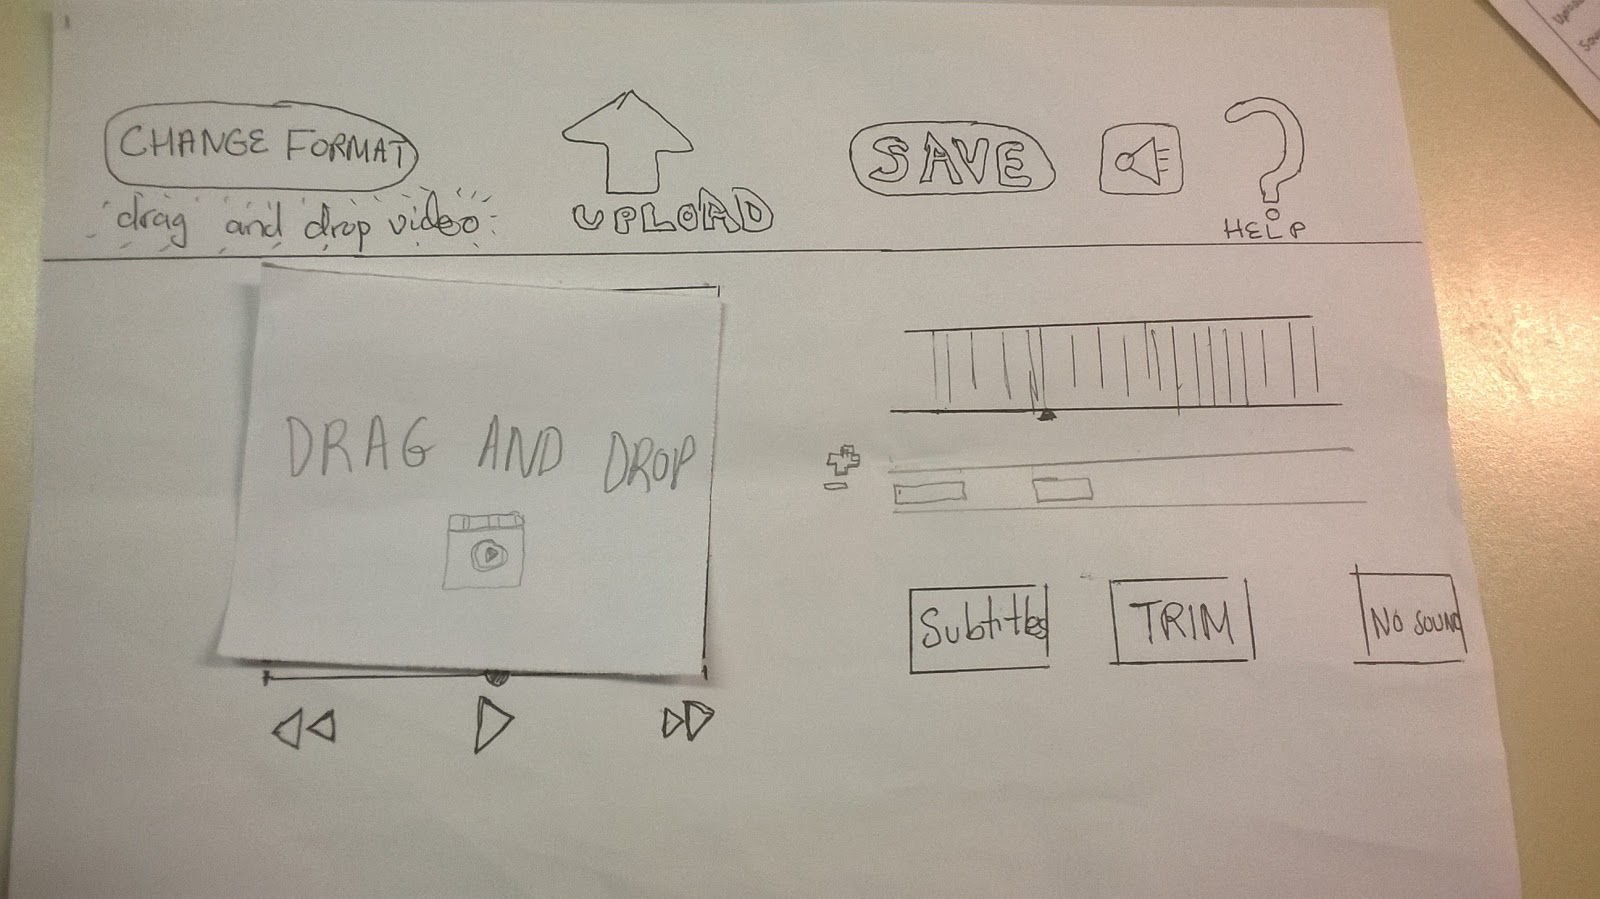
\includegraphics[scale=0.15]{paper}
\caption{The paper prototype; a simple design that included all the main functionality. Clicking on a function would bring up an additional window that was also paper-based.}
\end{figure}

Figure 1 is the prototype that was presented to the client, the system administrator and two other members of the DCCT. A user test session was conducted with them. A paper-based mock-up was used in order to receive feedback in a way that is affordable and easy to improve on or provide alternative designs \cite{sefelin2003paper}. Three participants took part in the evaluation of figure 1. One of the participants was the system administrator, and the other two are staff members at DCCT. The outcome of this evaluation can be seen in section \ref{Paper Prototype}.

\subsubsection{Interactive Prototype}
Based on the feedback from the paper prototype, an interactive prototype was created using the software Balsamiq \cite{studios2011balsamiq}. This formed part of the first cycle. Through the HCI class, we received additional feedback regarding the design which went into the design shown in figure 2. As a module assignment, we chose to use our Honours project. For this design, fellow classmates and our lecturer were consulted.

\begin{figure} [h]
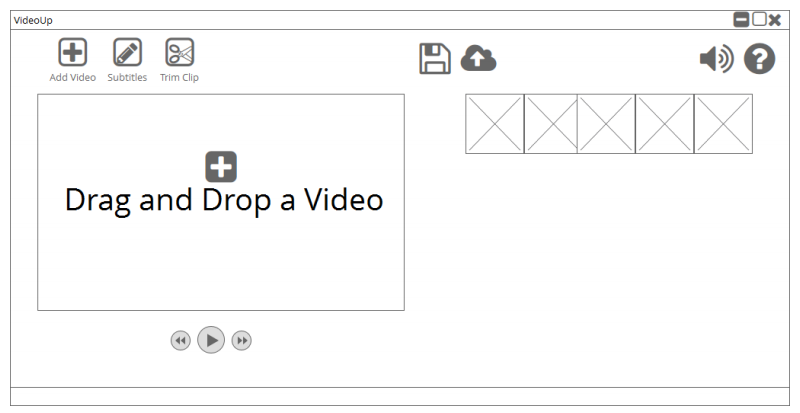
\includegraphics[scale=0.4]{interactive1}
\caption{The main window of the interactive prototype; this was based on the paper prototype with design improvements.}
\end{figure}

\begin{figure} [h!]
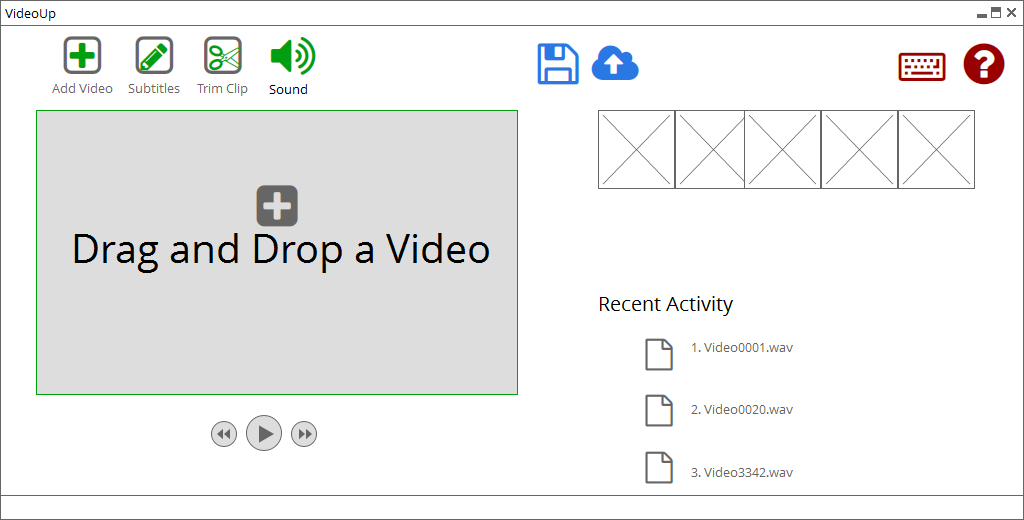
\includegraphics[scale=0.23]{interactive2}
\caption{Interactive prototype with colour added in order to group functionality}
\end{figure}

Figure 3 shows a slightly improved version of the interactive prototype. This simulation (interactive prototype) was better preferred over the paper prototype shown in figure 1, and this is mentioned in section \ref{Paper Prototype}. The sound icon was moved near the other main functionality (add, subtitles, trim). This was to emphasise that it is also a main functionality. Another addition was to add colour to the design. This was a way of highlighting and grouping functionality, which made identification easier.

\subsubsection{Cycle 2: Application development 1}
In the second cycle the first iteration of development began. The priority was on functionality at this point in time. The application was developed to trim, add metadata and convert a video. Audio could be removed as an option. As previously mentioned, this was presented to DCCT. Feedback from this meeting can be viewed from the Minutes of Meeting dated 30 July 2015\footnote{\href{http://people.cs.uct.ac.za/~nzxlub001/documents/Meryl-2015-07-30.pdf}{cs.uct.ac.za/$\sim$nzxlub001/documents/Meryl-2015-07-30.pdf}}. Below, in figure 4, is the computer design:

\begin{figure} [h]
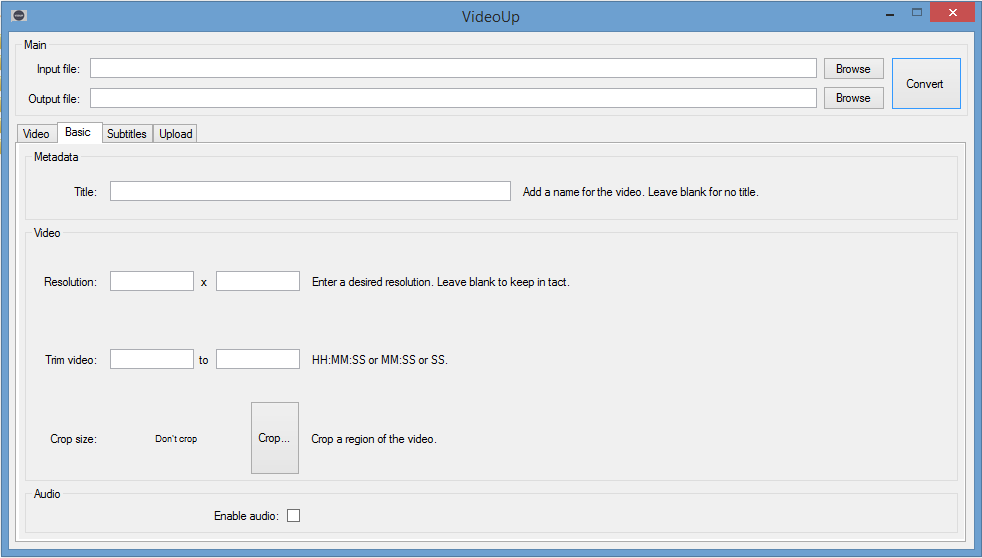
\includegraphics[scale=0.33]{dev1}
\caption{VideoUp first development. The open and save functions were located on top. Functionality was broken up into tabs in the lower third of the interface. The convert button was located at the top-right.}
\end{figure}

The input for the resolution and video trim left too much room for arbitration: any size could be put in for resolution, and the construct was not explained properly. Also, input validation had not been done yet. The trim video option was a little clearer, although input could be handled differently. The crop option was not fixed; it did not maintain standard ratios, so a user can make the aspect of the video be anything which could be a problem. Two aspects of design had not been addressed yet in this design: affordances and constraints. For example, the option for resolution was not clearly explained in the label. And there was no indicator as to how it worked. Additionally, input was in text, which meant that incorrect input was likely to occur. Norman's affordances \cite{mcgrenere2000affordances} said that clues should be provided as to how something works, and restrictions for the user to enter valid input.
It was mentioned at the presentation that the state of the conversion progress bar was unnecessary. It contained information which was irrelevant to the user, and should be removed. Removing this information would prevent the user from trying to understand information they may assume to be important, which was not for them \cite{volker2004thoughts}.

\subsubsection{Cycle 3: Application development 2}
The third cycle was the second iteration, which looked at incorporating further constraints. The function added to this iteration was the subtitle interface. Once these new additions were made, it was presented to the DCCT. Feedback from this presentation can be viewed from the Minutes of Meeting dated 17 September 2015\footnote{\href{http://people.cs.uct.ac.za/~nzxlub001/documents/Meryl-2015-09-17.pdf}{cs.uct.ac.za/$\sim$nzxlub001/documents/Meryl-2015-09-17.pdf}}.

\begin{figure} [h]
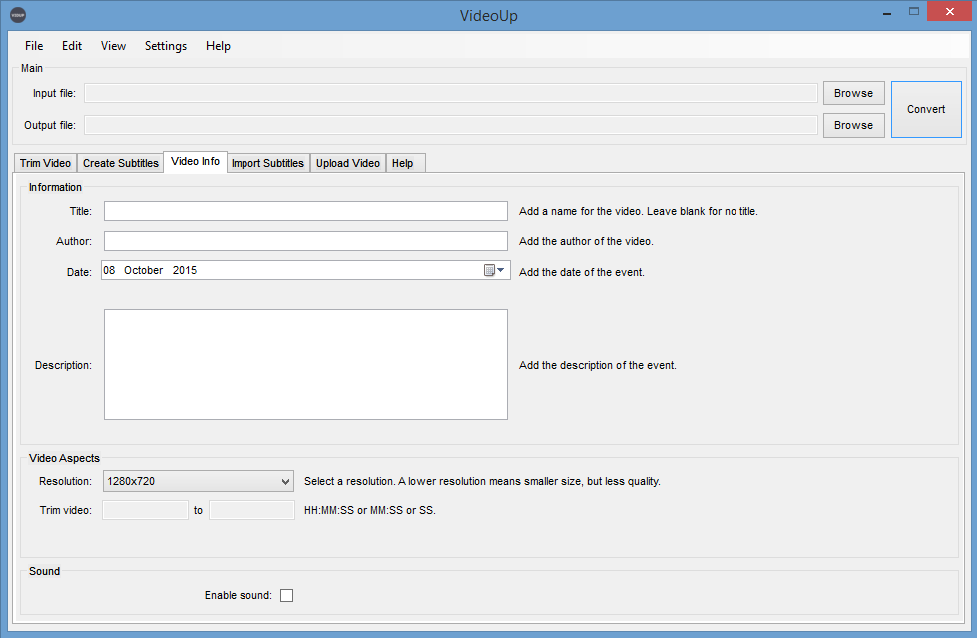
\includegraphics[scale=0.33]{dev2}
\caption{VideoUp second development. Additional tabs were added, including the subtitle and upload tabs. The navigation bar at the top was added, however no functionality had been implemented yet.}
\end{figure}

Additional tabs were created to make some of the functionality easier to use. For example, the trim option was simply done by placing the media player where you wanted the trim to start, and clicking the set start time button. A subtitle interface was added. However, it was noted that it was complicated confusing to use. The resolution option was now a drop-down of four different options instead of typing in the resolution. This reduced the chance of invalid errors, and creating a frame size that would not be fully understood by the user.

\subsubsection{Cycle 4: Application development 3}
The third iteration had a complete redesign in the interface. Colour was added and icons introduced. This is in keeping with the concept from the interactive prototype. The icons that have been emphasised in this design are the input, output and subtitle ones. They have been grouped together since they were similar options. The convert button stands out from the rest, so that it was easier to locate. The location of the help button followed the same rationale as the convert button.

\begin{figure} [h]
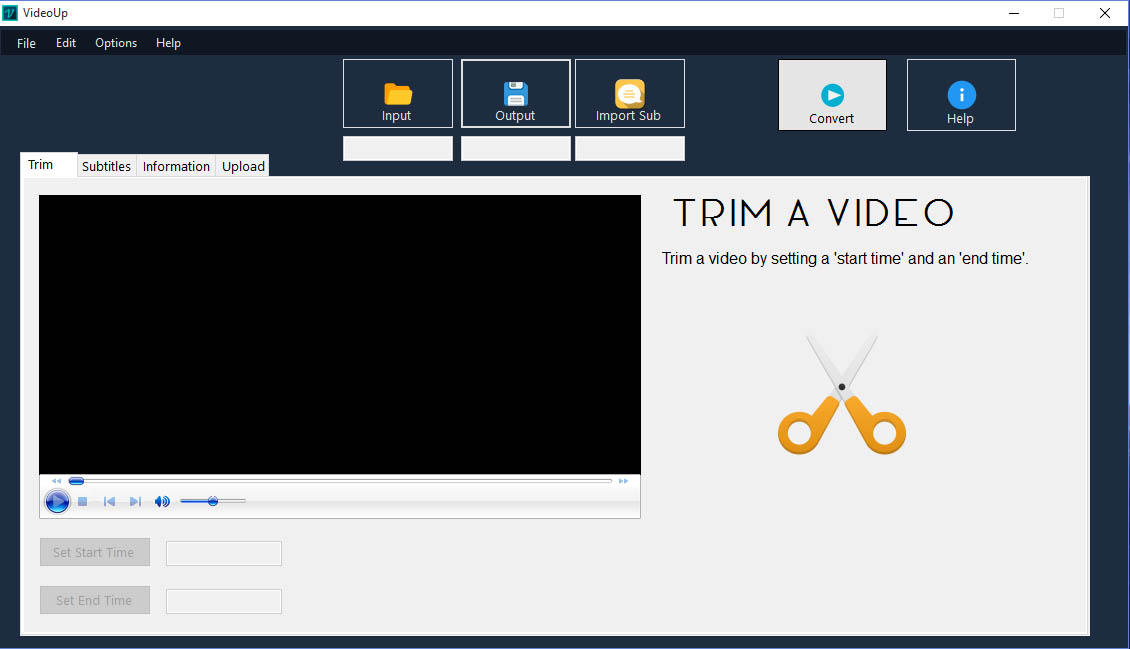
\includegraphics[scale=0.21]{dev3}
\caption{VideoUp third development. The open, save, convert and help buttons were emphasised by being placed on top.}
\end{figure}

Apart from input validations, the other functionality was simplified. A file menu strip was added, although the only buttons working were File and Help at this point. The colour adds an appeal to the application, and helps with identifying functionality along with the use of icons, as seen in figure 6. Two principles were considered here: least astonishment and least effort. Least astonishment looks at providing common behaviour for an application \cite{isaksen2006verification}. For example, opening and saving a video was presented in the same manner. Trimming a video was similar to creating a subtitle, with the subtitle interface requiring more steps to perform. Least effort is about performing tasks with as little effort as possible \cite{volker2004thoughts}. This tied in with the desire to keep the interface simple.

\subsubsection{Application development 4}
The fourth iteration had some minor UI changes. These changes were based on informal feedback received whilst at DCCT, and ones discussed within the team. Additionally, the help section videos were included here. The help section videos were recorded at DCCT, with the help of an interpreter. This design was presented to the DCCT through a user-test session, and comments recorded in section \ref{Results Findings}.

\begin{figure} [h]
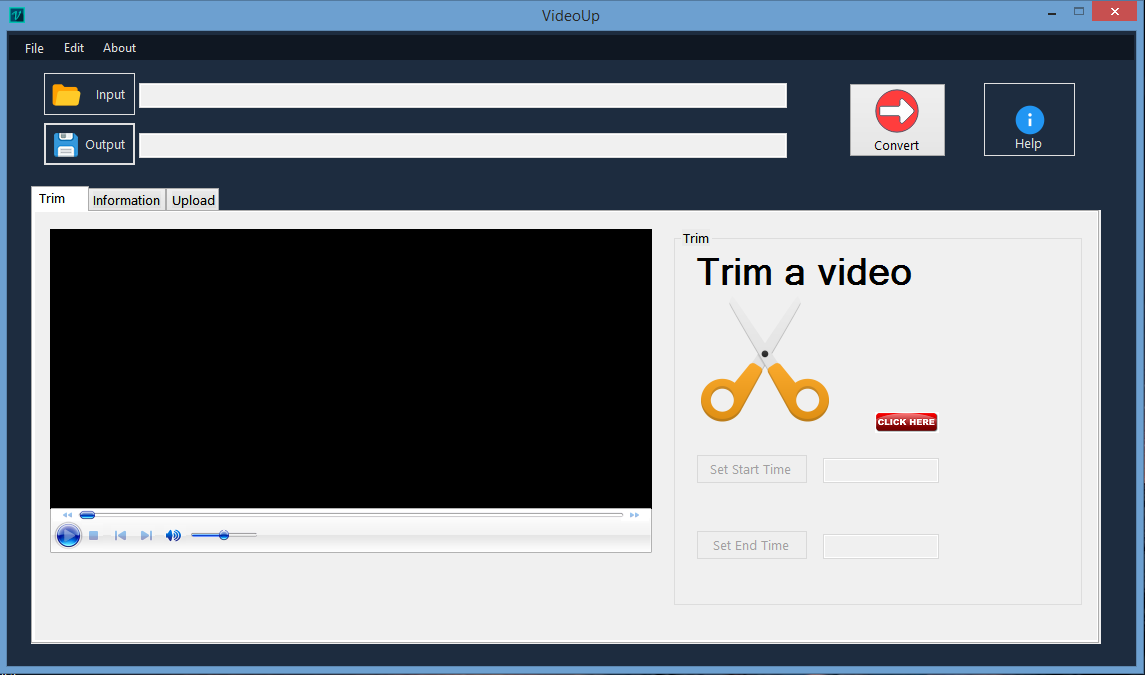
\includegraphics[scale=0.28]{dev4}
\caption{VideoUp fourth development. The open and save elements were returned to the one in cycle 2. Only the convert and help button were emphasised here.}
\end{figure}

For Input and Output, the file path box was brought back. This helped a user know the video file name, and where it is stored. Also, the import subtitle option was returned to the Information tab. The subtitle function was moved to the file menu strip. This was because the new subtitle interface would not fit into the tabbed viewing, so it was placed in a different window.

\section{Results and Findings}\label{Results Findings}
After the four qualitative design cycles a summative evaluation of the application was performed \cite{andrews2008evaluation}. Two user testing sessions were setup with three participants from DCCT. They were given a set of tasks on one or more of the application interfaces. The data received from these sessions was collected and analysed, in order to determine how the interface can be further improved. The second user test sessions also made use of a questionnaire, where participants were asked to rate components of the interface.

\subsection{Usability Test - Paper Prototype}\label{Paper Prototype}
The usability of a system is important when designing and developing an application. Not only that, but learnability also needs to be considered: how much of the application the user needs to become familiar with, and how long it takes to do so.

The first usability test was done in the form of a paper prototype, as outlined in the previous section. A Wizard of Oz approach was used \cite{arnowitz2010effective}. This is an interactive method of prototyping. One person acts as the computer, simulating each interaction decision a participant makes. Another person drives the process, by giving instructions and assisting participants where needed. A sample of 3 members of the DCCT were involved. These are the members who participate in the International Computer Driving License (ICDL) lessons that take place at DCCT every Thursday. Although there were few participants, the focus here was on collecting qualitative data. One of the members was experienced with computers, since he is a system administrator at DCCT. The other two members were familiar with the basic use of a computer.

\subsection*{Procedure}
The users were asked to:
\begin{itemize}
  \item Add a video to the interface, where they could do this by selecting the "Find Video" option or dragging the video onto the application
  \item Make a trim of the selected video with a specified length
  \item Add subtitles to the selected video
  \item Remove audio from the selected video
  \item Save the project file into a directory
  \item Upload the video, where they would add a description to the video and proceed by clicking the Submit button to upload
\end{itemize}

From the project, two members were in charge of facilitating the user test session. One project member acted as the system, by simulating actions when a user wanted to perform a certain action. The other project member outlined what needed to be done, and assisted when necessary.

The three participants mentioned that they liked the simplicity of the design, and found the UI elements relatively easy to interpret. However, they found that the paper prototype was a little complicated. This is because it was hard to simulate computer interactions using pieces of paper.

\subsection*{Results}
The three participants mentioned that they liked the simplicity of the design, and found the UI elements relatively easy to interpret. However, they mentioned that a software version would have been better \cite{sefelin2003paper}. Additionally, the system administrator was the only one who had experience with conversion and editing tools. The system administrator performed the tasks quicker compared to the other two participants.

There was some confusion that was a result of the design approach itself. The trim and subtitle functions were difficult to interpret for the participants, so additional help was needed to complete these tasks. The participants have worked with computers as previously mentioned, so they found UI elements that were annotated with Sign Language to be unnecessary.

\subsection*{Discussion of results}
The participants were calm at the beginning of the session. Towards the end, the system administrator wanted to increase the pace as he was familiar with this kind of software interface. The other two participants took a bit more time as they were new to this kind of interface. The system administrator pointed out that the Sign Language interpretations of UI elements were unnecessary, and the other two participants agreed. He mentioned that, although they are Deaf, they can understand the jargon associated with UI elements.

At some instructions we may have over communicated the instructions, which resulted in the users knowing exactly what to do. Instead, those few instructions should have been simply stated, so that we could observe user behaviour before assisting. This may have affected our results.

\subsection{Usability Test - Developed Application}\label{Developed Application}
The second usability test was done on the fourth iteration. A sample of 3 members of DCCT were asked to participate. Again, one of the members was experienced with computers, since he is a system administrator at DCCT. The other two members were familiar with the basic use of a computer. The full results of this session can be viewed on the webpage\footnote{\href{http://people.cs.uct.ac.za/~nzxlub001/documents/usabilityTestResults.pdf}{cs.uct.ac.za/$\sim$nzxlub001/documents/usabilityTestResults.pdf}}.

\subsection*{Procedure}
The users were asked to:
\begin{itemize}
  \item Trim a video
  \item Create subtitles
  \item Add video metadata
  \item Convert a video with the created subtitles
  \item Upload the videos
  \item Organise the videos using the file manager
\end{itemize}

\subsection*{Results}
For the trim functionality, all three participants performed well. They said that it was easy to trim a video, and the instructions provided were clear. The next function was adding subtitles. Once the first subtitle had been entered, they understood how it worked, and proceeded to enter a second and a third subtitle. They mentioned that it would be good to be able to view subtitles on the media player, and that colour could be used to highlight key buttons on the subtitle interface.

In the video information section, they mentioned that the resolution field was not clear. There are four options to choose from here, but the resolutions (1920x1080 for example) did not make outright sense. They also mentioned that the remove sound option was a little confusing. Perhaps the wording of it could have been phrased differently to avoid confusion. Importing subtitles was fine; participants managed to add the subtitles they created to the video they were using.

When it came to uploading, there were a few issues. Only one of the three participants got the YouTube authentication page, in order to login and upload the video. This did not happen for the other two, so they were puzzled. Additionally, the feedback message came in intervals, so in-between the participants did not know if the video was still uploading or not.

Finally, the file manager did not work well in this test session.

\subsection*{Discussion of results}
  \noindent
  Firstly: the file manager did not work well as mentioned in the results. It failed to start up when the participants attempted to use it. This could possibly be a compatibility issue with the computer used for the testing session. Also, the upload progress was intermittent, so there were times participants were unaware if the upload was still ongoing or not.\\
  
  \noindent
  Trim: All the participants were able to trim the video successfully. The first participant did not trim according to the specification set out in the test.\\
  
  \noindent
  Subtitle: Initially, two participants struggled to find where the subtitle interface was located. They understood how to create a subtitle, as the functionality was similar to that of trim.\\
  
  \noindent
  Information: Participants did fairly well in this section. One participant was a little confused with the import subtitle function, but made use of the help function.\\
  
  \noindent
  Upload: All participants mentioned that, because there was no proper progress indicator, it was hard to see whether the video was uploading or not, and if that upload was successful or not.\\
  
  \noindent
  Help videos: Participants found this feature to be helpful. The videos were accessible on-demand, while being available only when needed. They were not laid out in the entire interface.

\subsection{User Acceptance Test}
The User Acceptance Test helped to serve two purposes: it checked whether all the functionality intended worked, and it was a way of getting the user familiar with the core functionality of the application. This test was done at the end of the development iteration \cite{boltonuser}, and served as an evaluation of the application in its current state.

\subsection*{Requirements}
These were the requirements that were considered in the User Acceptance Test.

\begin{table} [ht]
\caption{User Acceptance Test Criteria Matrix}
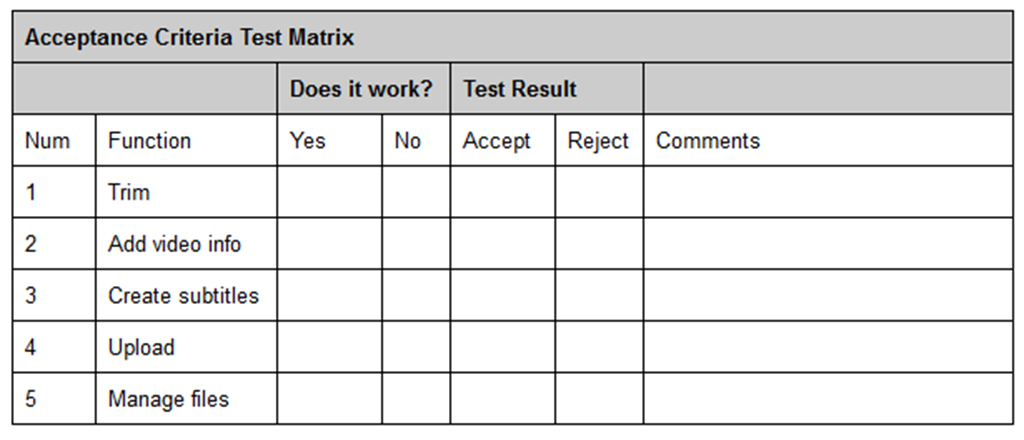
\includegraphics[scale=0.23]{uat}
\end{table}

\subsection*{Results}
Table 1 displays the criteria that was used to rate the application. The participants gave the application a pass rating. Although they gave the application a greenlight, they did provide useful feedback on how it can be improved. The concerns centred around the upload and file management functionality, as explained in section \ref{Developed 
Application}. Apart from that, the users were satisfied with the trim, video info and subtitle functionalities. More on these results can be seen on the webpage.

\subsection*{Discussion of results}
The application was evaluated, and determined to be a success. The participants believe that the functionality set out in the application worked as intended. The feedback from them was noted, and it applies to two of the five functionalities. With regards to the upload function, the progress indicator could be improved by: adding a loading spin wheel. This would give a clear indicator of progress, and would suspend the rest of the application until the upload is complete. The YouTube login should be reset for each video upload, to avoid users making use of another person's account. Once this is done, the link can be taken from YouTube and placed onto the DCCT website. The file manager did not work well on the computer where the user testing took place. However, it works well on other windows 7 machines tested in the same DCCT lab. It is possible that this is a computer-specific problem, not a general one.

\section{Conclusion}
The proposed application is VideoUp: An editing, file managing and upload tool. It has been developed to assist the Deaf Community of Cape Town with the editing and managing of current and future recordings of events that they hold or are a part of. The back-end of the application focused on providing the core functionality, while the front-end dealt with the presentation of the interface, the capturing of user input and the inclusion of Sign Language.

The key-questions in the design of the interface were:
\begin{enumerate}
  \item How can the interface be kept simple but effective?
  \item How feasible is it to add a help section that is driven by Sign Language?
\end{enumerate}

In the presentation of Figure 4 (application development 1), the client and system administrator mentioned that technical aspects should be clear and explained. Also, feedback to the user should not contain anything that is not useful to them. This is evident in the third and fourth iteration, where the interface was cleaned and refined. Participants responded positively to this, and mentioned how things were kept simple, and had visual feedback. This is because the environment, level of computer skills and experience were all taken into account. At the same time, oversimplifying the application was avoided so that the user is not treated as incompetent or unable.

The user testing session making use of the final interface design had the Sign Language help section included. The motivation here was to have an option where the user may interact in their preferred language of choice. The videos were recorded with an interpreter and a member of the DCCT. Participants found this to be a useful feature in the user test session.

\section{Acknowledgments}
I would like to thank our supervisor Prof. Edwin Blake for the guidance and commitment he showed throughout this project. Thanks also go to our client Ms. Meryl Glaser for helping us with our engagement with the DCCT. I would also like to thank the members of DCCT, and Mr. Richard Pelton in particular, for the help and willingness they showed throughout this project. Special thanks go to Dr. Melissa Densmore, Sifiso Duma, Montlamedi Maikano, George Ng'ethe and Bhavana Harrilal.

\medskip

\bibliographystyle{acm}
\bibliography{sigproc}

\end{document}